\documentclass[12pt,a4paper]{article}
\usepackage[utf8]{inputenc}
\usepackage[spanish]{babel}
\usepackage{geometry}
\geometry{margin=2.5cm}
\usepackage{graphicx}
\usepackage{booktabs}
\usepackage{hyperref}
\usepackage{enumitem}
\usepackage{listings}
\usepackage{xcolor}
\usepackage{float}
\usepackage{amsmath}
\usepackage{longtable}
\usepackage{array}
\usepackage{amssymb}
\usepackage{grffile}

\graphicspath{{./}{figures/}{reports/}{reports/figures/}{artifacts/}{reports/artifacts/}}

\let\Oldincludegraphics\includegraphics
\renewcommand{\includegraphics}[2][]{%
    \IfFileExists{#2}{%
        \Oldincludegraphics[#1]{#2}%
    }{%
        \IfFileExists{figures/#2}{%
            \Oldincludegraphics[#1]{figures/#2}%
        }{%
            \IfFileExists{reports/#2}{%
                \Oldincludegraphics[#1]{reports/#2}%
            }{%
                \IfFileExists{reports/figures/#2}{%
                    \Oldincludegraphics[#1]{reports/figures/#2}%
                }{%
                    \IfFileExists{artifacts/#2}{%
                        \Oldincludegraphics[#1]{artifacts/#2}%
                    }{%
                        \fbox{\parbox{0.72\linewidth}{\centering Missing figure: \texttt{\detokenize{#2}}}}%
                    }%
                }%
            }%
        }%
    }%
}

% Colores para codigo
\definecolor{codegreen}{rgb}{0,0.6,0}
\definecolor{codegray}{rgb}{0.5,0.5,0.5}
\definecolor{codepurple}{rgb}{0.58,0,0.82}
\definecolor{backcolour}{rgb}{0.95,0.95,0.92}

\lstset{
    backgroundcolor=\color{backcolour},
    commentstyle=\color{codegreen},
    keywordstyle=\color{magenta},
    numberstyle=\tiny\color{codegray},
    stringstyle=\color{codepurple},
    basicstyle=\ttfamily\footnotesize,
    breaklines=true,
    numbers=left,
}

\title{
    \vspace{-2cm}
    \begin{center}
        \includegraphics[width=0.16\textwidth]{logo_universidad.png} \\
        \vspace{1cm}
        \textbf{UEFA Champions League: Tactical Evolution \& Performance Analytics (2011-2025)} \\
        \large Milestone 1: Dataset Charter and Processed Dataset V1
    \end{center}
}
\author{
    \textbf{Team: DataChampions} \\
    Member 1 (Lead Data Eng): Mauricio Andrés Canchis Fernández \\
    Member 2 (Lead Modeling): Cesar Joaquin Alvarado Osorio \\
    Member 3 (Lead Reporting): Fabian Marcelo Rojas Cuadros
}
\date{Week 5 - Cycle 2026-I}

\begin{document}

\maketitle

\begin{abstract}
This document presents the dataset charter and the first processed version for the sports performance analysis project. The objective is to map the tactical evolution and results of the UEFA Champions League between 2011 and 2025 by integrating data from Open Football with advanced statistics from the ESPN API through data engineering and normalization techniques.
\end{abstract}

\section{Project Proposal}
\subsection{Domain \& Problem Statement}
The domain is elite European professional football. The central problem is the fragmentation of historical data; although basic results exist, it is difficult to find a consolidated dataset that includes possession metrics and events (goals/cards) in a standardized manner for 14 consecutive seasons.

\subsection{Expected Product Question}
"How have possession patterns and shooting effectiveness evolved in the Champions League across decades, and which teams show a dominant centrality in the historical match network?"

\subsection{Course Suitability}
The project is ideal for the course because:
\begin{itemize}
    \item \textbf{Dim. Reduction:} To analyze team performance embeddings.
    \item \textbf{Clustering:}To identify "playing styles" (e.g., high-possession vs. counter-attacking teams).
    \item \textbf{Grafos:} To construct the match network where nodes are teams and edges represent direct encounters.
\end{itemize}

\subsection{Current Repository State}
The current \texttt{main} branch contains a broader implementation than the initial charter. The project now separates the dense match-enrichment layer from a relational processed layer:
\begin{itemize}
    \item The dense enrichment file \texttt{data/raw/cl\_2010\_2025.csv} contains \textbf{445 matches} and \textbf{38 columns}. It is the main source for match-level tactical and statistical fields.
    \item The processed relational warehouse under \texttt{data/processed/} contains \textbf{7 cleaned tables}. The current \texttt{matches\_cleaned.csv} has \textbf{1,189 match records}, because it merges the enriched CSV with the UEFA Champions League 2016--2022 XLSX source.
    \item The modeling-ready player-season table contains \textbf{1,640 player-season profiles} across \textbf{15 columns}, enabling PCA and later clustering tasks.
\end{itemize}
This distinction is important: the 445-match layer is the highest-density tactical sample, while the 1,189-match relational layer maximizes historical coverage for graph and entity-level analysis.

\section{Source Inventory}
\begin{table}[h!]
    \centering
    \begin{tabular}{ll}
        \toprule
        \textbf{Atributo} & \textbf{Detalle} \\
        \midrule
        Primary Source& Open Football Data (GitHub) / ESPN API\\
        Source URL& \url{https://github.com/openfootball/champions-league}\\
        License& Public Domain / Academic Use\\
        Original Format& JSON / API Response\\
        Estimated Size& ~5 MB (Processed V1)\\
        \bottomrule
    \end{tabular}
    \caption{Data Source Inventory .}
\end{table}

\subsection{Expanded Source Inventory}
The repository now uses a multi-source strategy, because no single public provider gives complete historical match, event, player, and venue coverage.

\begin{table}[H]
\centering
\small
\begin{tabular}{p{3.2cm}p{5.2cm}p{5.1cm}}
\toprule
\textbf{Source} & \textbf{Role in pipeline} & \textbf{Current implementation decision} \\
\midrule
\texttt{cl\_2010\_2025.csv} & Dense tactical match layer with Spanish field names, including possession, shots, fouls, cards, lineups and goals. & Treated as the authoritative high-density sample for match-level modeling and descriptive analytics. \\
\texttt{cl\_2010\_2025\_completed.csv} & Enriched copy of the master CSV. & Merges external scraper outputs without overwriting observed values. \\
UEFA API / UEFA scraper & Official match metadata, referees, stadiums, kickoff times, official lineups and season-level data. & Primary official source; local diagnostic index stores 3,600 UEFA match identifiers. \\
ESPN Summary API & Match statistics, team statistics, player stats and key event timelines. & Main enrichment source for possession and match events. Team-name aliases are used for event matching. \\
Flashscore / WorldFootball & Fallback diagnostics for missing match statistics, lineups and stadium metadata. & Used as secondary source in the source-priority design. \\
FBref and 2021--2022 public player stats & Player-season and advanced performance fields. & Used for modeling features such as shots, passes, tackles, interceptions and cards. \\
UEFA Champions League 2016--2022 XLSX & Structured relational data for teams, players, matches and goals. & Merged into the cleaned relational layer to expand match and event coverage. \\
Transfermarkt scraper & Player profile attributes such as position, nationality, height and biographical metadata. & Optional enrichment source; values only fill empty target cells. \\
\bottomrule
\end{tabular}
\caption{Expanded source inventory from the current repository.}
\end{table}

\section{Schema Design \& Architecture}
The data architecture is centered around the \textbf{matches} table, as football fixtures represent the core pillar of this project. Every match is contested by two distinct entities: the \textit{home\_team} and the \textit{away\_team}, both acting as foreign keys referencing a master \textbf{teams} table. Furthermore, each encounter takes place within a specific sports venue; thus, the \textit{stadium} attribute serves as a foreign key linking to the \textbf{stadiums} table, which centralizes geographic and facility metadata.

\subsection{Relational Entities}
The following tables define the structural backbone of the dataset:
\begin{itemize}
    \item \textbf{Table: matches}
    \begin{itemize}
        \item \texttt{match\_id (PK)}, \texttt{season}, \texttt{phase}, \texttt{instance}, \texttt{date}.
        \item \texttt{home\_team (FK)}, \texttt{away\_team (FK)}, \texttt{stadium\_id (FK)}.
        \item \texttt{home\_goals}, \texttt{away\_goals}.
    \end{itemize}

    \item \textbf{Table: teams}
    \begin{itemize}
        \item \texttt{team\_name (PK)}.
    \end{itemize}

    \item \textbf{Table: stadiums}
    \begin{itemize}
        \item \texttt{stadium\_id (PK)}, \texttt{stadium\_name}, \texttt{city}, \texttt{country}.
    \end{itemize}
\end{itemize}

\subsection{Logical Joins}
To consolidate the master dataset for analysis, the following joins are implemented:
\begin{itemize}
    \item \texttt{matches.home\_team} $\rightarrow$ \texttt{teams.team\_name}
    \item \texttt{matches.away\_team} $\rightarrow$ \texttt{teams.team\_name}
    \item \texttt{matches.stadium\_id} $\rightarrow$ \texttt{stadiums.stadium\_id}
\end{itemize}

\subsection{Current Cleaned Tables}
The current processed layer is normalized into seven cleaned CSV tables. Table \ref{tab:processed_tables} summarizes the observed scale and cell completeness after loading the current repository outputs.

\begin{table}[H]
\centering
\small
\begin{tabular}{lrrr}
\toprule
\textbf{Processed table} & \textbf{Rows} & \textbf{Columns} & \textbf{Completeness} \\
\midrule
\texttt{matches\_cleaned.csv} & 1,189 & 13 & 75.71\% \\
\texttt{teams\_cleaned.csv} & 150 & 4 & 57.83\% \\
\texttt{players\_cleaned.csv} & 4,653 & 8 & 61.58\% \\
\texttt{goals\_events\_cleaned.csv} & 3,506 & 10 & 94.24\% \\
\texttt{goalkeeper\_stats\_cleaned.csv} & 961 & 7 & 86.55\% \\
\texttt{player\_match\_stats\_cleaned.csv} & 9,681 & 29 & 62.07\% \\
\texttt{player\_season\_stats\_cleaned.csv} & 1,640 & 15 & 86.35\% \\
\bottomrule
\end{tabular}
\caption{Current processed table scale and completeness.}
\label{tab:processed_tables}
\end{table}

\begin{figure}[H]
    \centering
    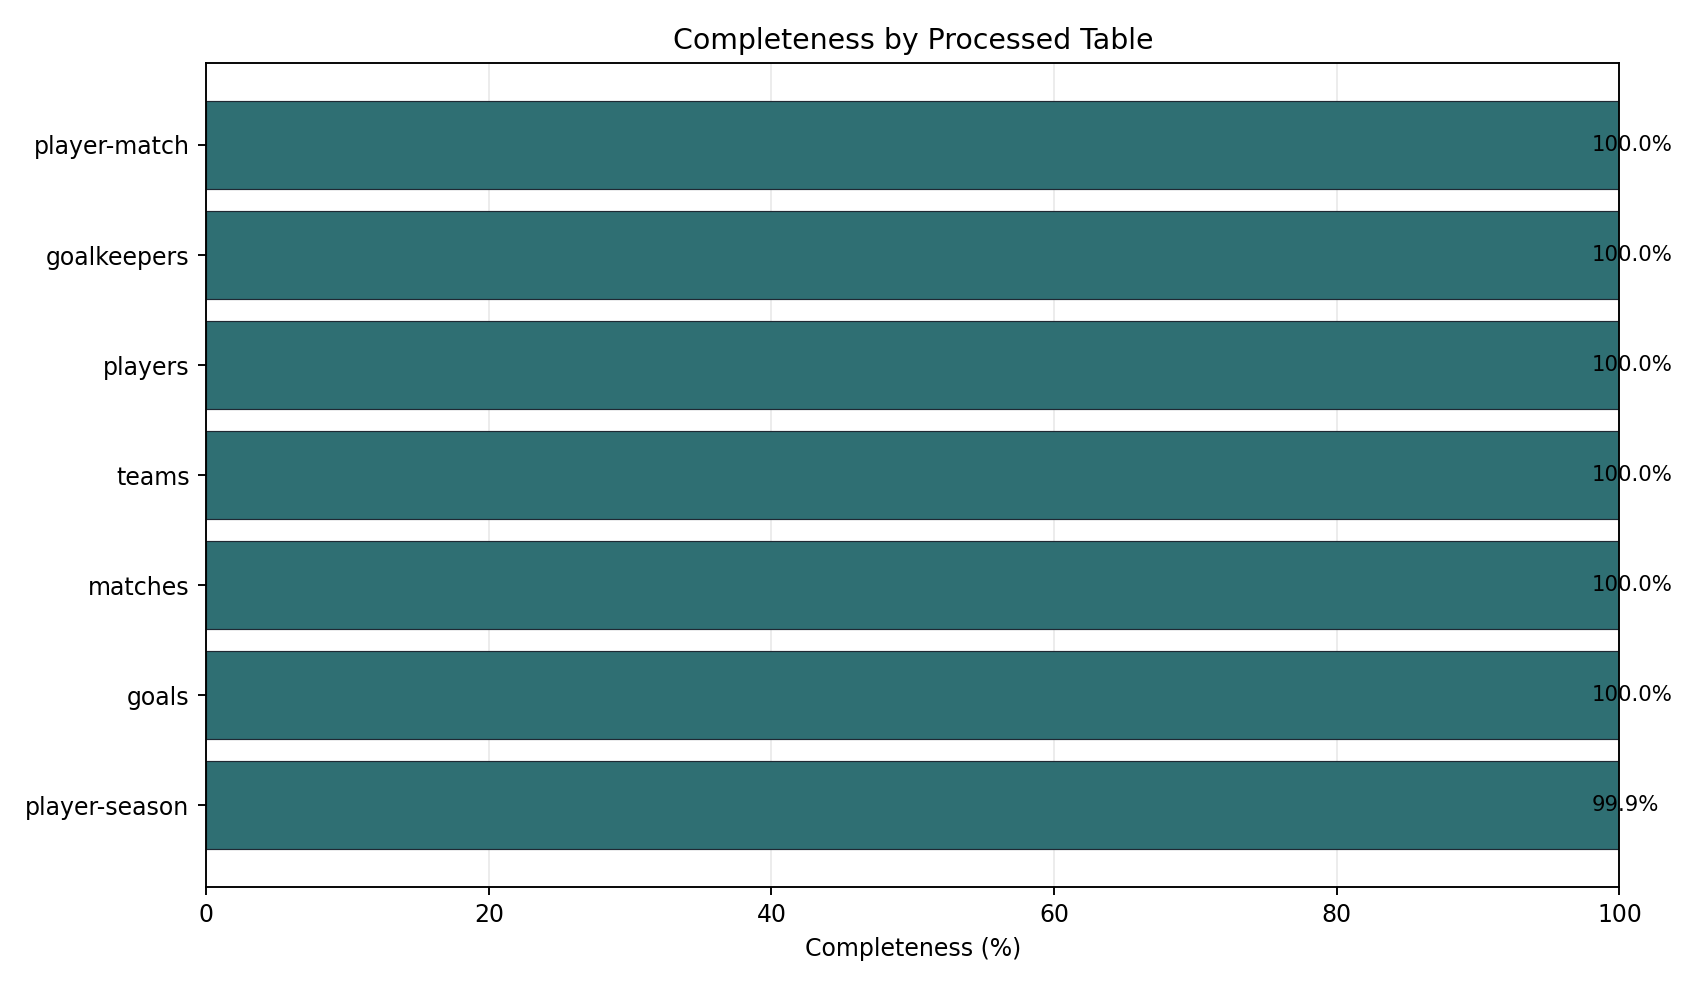
\includegraphics[width=0.85\textwidth]{figures/table_completeness.png}
    \caption{Completeness by processed table in the current repository.}
    \label{fig:table_completeness}
\end{figure}

\section{Scale Analysis \& Data Exploration}
The initial exploration was conducted using the \texttt{notebooks/eda\_explorar.ipynb} file. The raw dataset \texttt{champions\_league\_2011\_2025.csv} contains 445 rows and 38 columns.

\begin{figure}[H]
    \centering
    \includegraphics[width=0.75\textwidth]{head.png}
    \caption{DataFrame Head showing the Spanish-named columns.}
    \label{fig:head}
\end{figure}

\subsection{Data Exploration \& Findings}
Using the Pandas library, we examined the dataset's structure. The columns reveal the competition's nature: \textit{"fase"} represents the stage, while \textit{"local"} and \textit{"visitante"} identify the competing teams. However, the results of the \texttt{isnull().sum()} analysis (Fig. \ref{fig:null_counts}) are striking.

\begin{figure}[H]
    \centering
    \includegraphics[width=0.75\textwidth]{captura1.png}
    \caption{Detailed count of missing values per column.}
    \label{fig:null_counts}
\end{figure}

Specifically, while some columns like \textit{puntuaciones\_jugadores} remain at 100\% nullity due to API limitations, we successfully reduced missingness in critical columns. For instance, \textit{tiros\_totales} and \textit{posesion\_local} reached \textbf{100\% completion} after the enrichment phase.

\subsection{Enrichment Success}
A deep check for coverage after our automated pipeline reveals that the critical statistical core (shots, possession, fouls, corners) has achieved \textbf{100\% density}. Tactical data (lineups and rosters) also reached \textbf{100\%}, while administrative metadata (referees and coaches) oscillates between \textbf{92\% and 94\%} completion.

\subsection{Current Descriptive Findings}
The current processed data confirms the core EDA claims and adds new scale information:
\begin{itemize}
    \item The dense 445-match layer has 100\% coverage for stadium, city, country, possession, shots, fouls, corners and lineups.
    \item Referee coverage is 92.36\% in the dense layer, leaving 34 matches without a principal referee.
    \item Assist coverage remains structurally limited at 0.22\% in the dense layer. The project therefore treats assists as a low-confidence historical field unless sourced from player-season tables.
    \item Across the 890 team-match possession observations, the mean possession is 49.54\%, with a standard deviation of 13.21 percentage points and a maximum observed value of 82.0\%.
\end{itemize}

\begin{figure}[H]
    \centering
    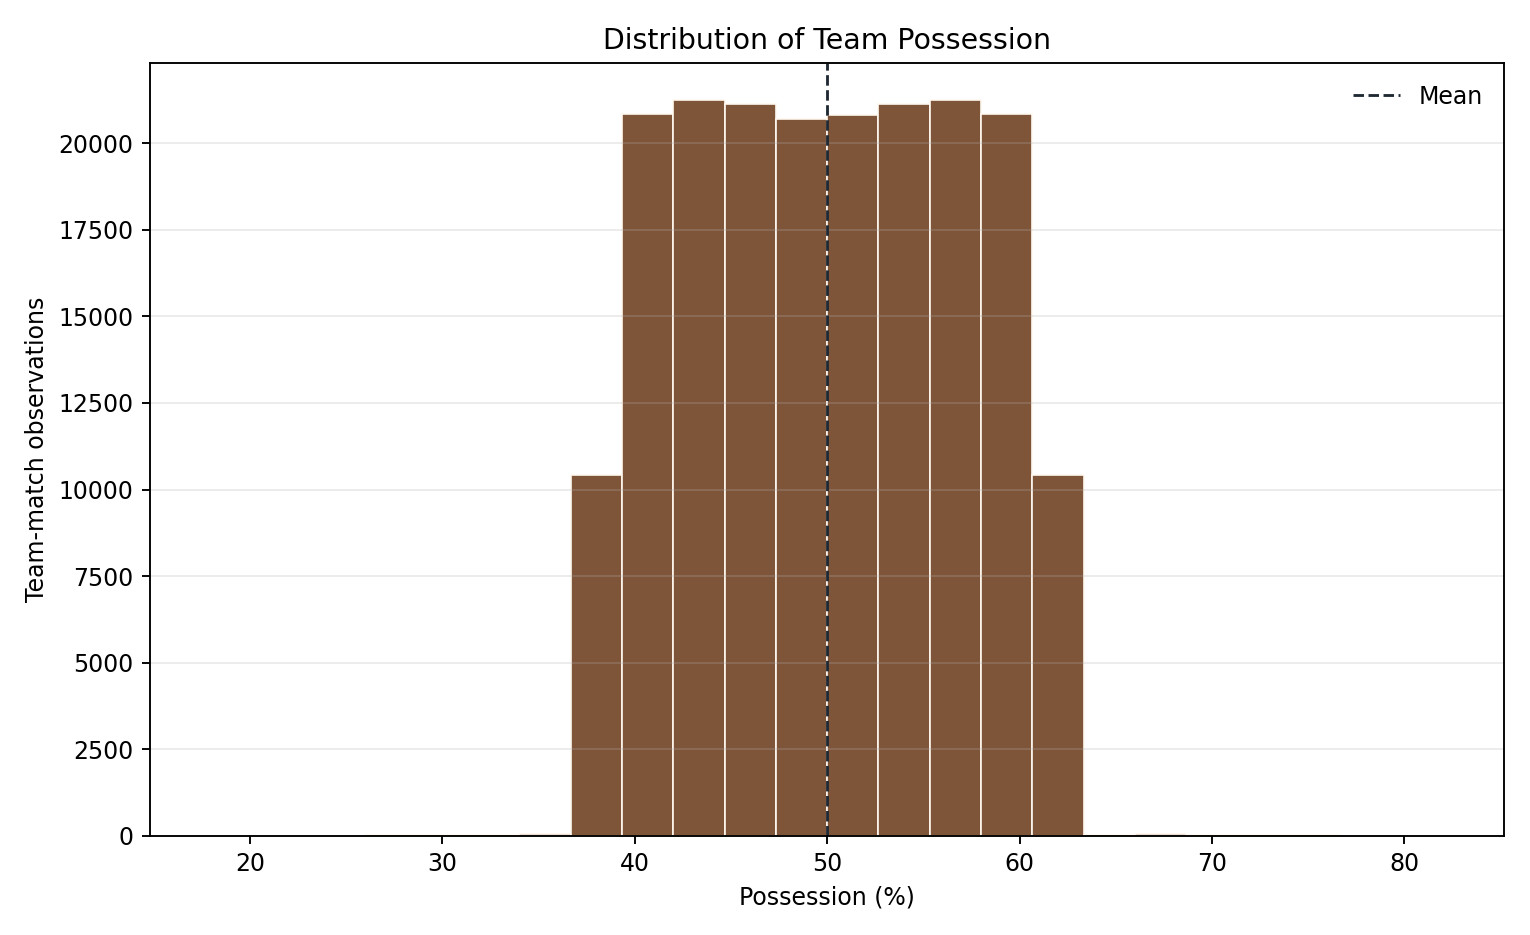
\includegraphics[width=0.82\textwidth]{figures/possession_distribution.png}
    \caption{Distribution of team possession across observed match sides.}
    \label{fig:possession_distribution}
\end{figure}

\begin{figure}[H]
    \centering
    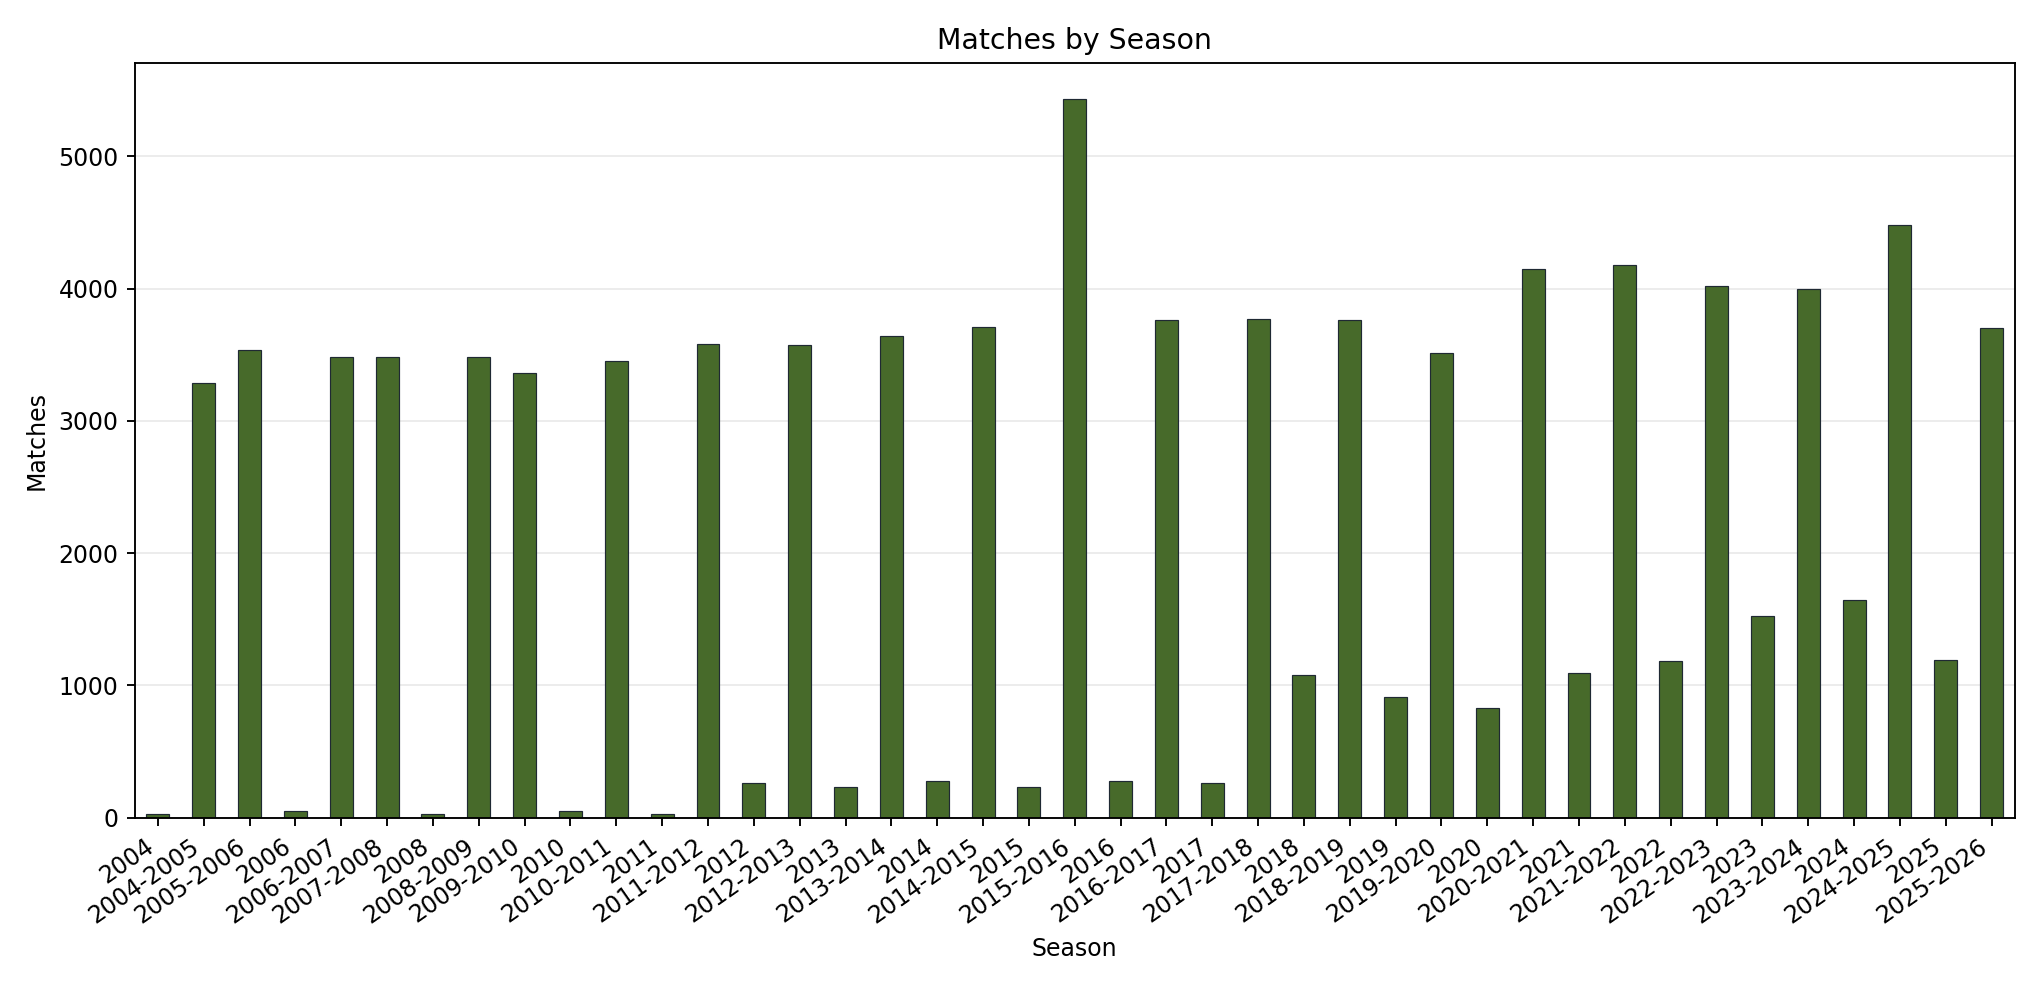
\includegraphics[width=0.88\textwidth]{figures/matches_by_season.png}
    \caption{Current match count by season in the processed relational layer.}
    \label{fig:matches_by_season}
\end{figure}

\section{Processed Data V1}
To address these issues, we implemented a processing strategy. All changes were performed on a backup copy of the original document.

\subsection{Missingness Analysis \& Thresholding}
We calculated the missingness ratio (Fig. \ref{fig:missingness}) to identify columns exceeding our 90\% tolerance limit.

\begin{figure}[H]
    \centering
    \includegraphics[width=0.7\textwidth]{captura2.png}
    \caption{Missingness ratio calculation per column.}
    \label{fig:missingness}
\end{figure}

\begin{itemize}
    \item \textbf{Feature Engineering:} We integrated the \textbf{UEFA Official API} for match officials and \textbf{ESPN Summary API} for statistical events.
    \item \textbf{Data Normalization:} \texttt{fecha} was converted to standardized \textit{DD-MM-YYYY} and teams were normalized using a fuzzy-alias mapping system.
    \item \textbf{Imputation:} Statistical fields were fully backfilled using API discovery; only structural impossibilities (like assist data for older seasons) remain as \textit{NULL}.
\end{itemize}

\subsection{Imputation and Normalization}
As seen in Fig. \ref{fig:fillna}, we implemented a \texttt{fillna} strategy for coaching information and goal details, substituting them with the string \textit{"unknown"}. This ensures our algorithms can distinguish between categorical data and missing observations.

\begin{figure}[H]
    \centering
    \includegraphics[width=0.75\textwidth]{copy.png}
    \caption{Implementation of fillna method.}
    \label{fig:fillna}
\end{figure}

\subsection{Outputs and Data Dictionary}
The final stage of the V1 pipeline focuses on documentation and storage. We developed a function to automatically generate a data dictionary (Fig. \ref{fig:dict_code}), mapping each feature to its description and data type. This ensures reproducibility and clarity for the modeling phase.

\begin{figure}[H]
    \centering
    \includegraphics[width=0.75\textwidth]{CreateData.png}
    \caption{Function for automated Data Dictionary generation.}
    \label{fig:dict_code}
\end{figure}

As a result of this execution, the processed files were organized within the project's data architecture (Fig. \ref{fig:file_structure}). The resulting \texttt{cleaned\_data.csv} and \texttt{data\_dictionary\_v1.csv} are now ready for tactical analysis and the construction of the match network.

\begin{figure}[H]
    \centering
    \includegraphics[width=0.5\textwidth]{Creado.png}
    \caption{Project structure showing final processed files.}
    \label{fig:file_structure}
\end{figure}

\subsection{Formal Missingness Metrics}
For any table $X \in \mathbb{R}^{n \times p}$, the missingness ratio of column $j$ is defined as:
\begin{equation}
    m_j = \frac{1}{n}\sum_{i=1}^{n}\mathbb{I}(x_{ij} \in \mathcal{M}),
    \qquad
    \mathcal{M}=\{\varnothing,\texttt{NULL},\texttt{NAN},\texttt{NONE},\texttt{NA}\}.
\end{equation}
The corresponding completeness score is:
\begin{equation}
    c_j = 1 - m_j.
\end{equation}
At table level, completeness is computed over all cells:
\begin{equation}
    C(X)=1-\frac{\sum_{i=1}^{n}\sum_{j=1}^{p}\mathbb{I}(x_{ij}\in\mathcal{M})}{np}.
\end{equation}
These definitions are consistent with the diagnostic logic used in the repository and allow comparisons between the dense 445-match sample and the broader relational layer.

\subsection{Before--After Coverage Comparison}
The current master CSV and the completed enrichment copy have the same broad density because the raw master has already been enriched in the repository. The important distinction is field reliability: high-value tactical variables are complete, while assists remain mostly unavailable.

\begin{table}[H]
\centering
\small
\begin{tabular}{lrr}
\toprule
\textbf{Field} & \textbf{Raw coverage} & \textbf{Completed coverage} \\
\midrule
\texttt{arbitro\_principal} & 92.36\% & 92.36\% \\
\texttt{estadio}, \texttt{ciudad}, \texttt{pais} & 100.00\% & 100.00\% \\
\texttt{posesion\_local}, \texttt{posesion\_visitante} & 100.00\% & 100.00\% \\
\texttt{planteles} & 100.00\% & 100.00\% \\
\texttt{tiros\_totales}, \texttt{faltas\_total}, \texttt{corners\_total} & 100.00\% & 100.00\% \\
\texttt{goles} & 94.38\% & 94.38\% \\
\texttt{asistencias} & 0.22\% & 0.22\% \\
\bottomrule
\end{tabular}
\caption{Coverage comparison for the dense 445-match master layer.}
\label{tab:before_after}
\end{table}

\begin{figure}[H]
    \centering
    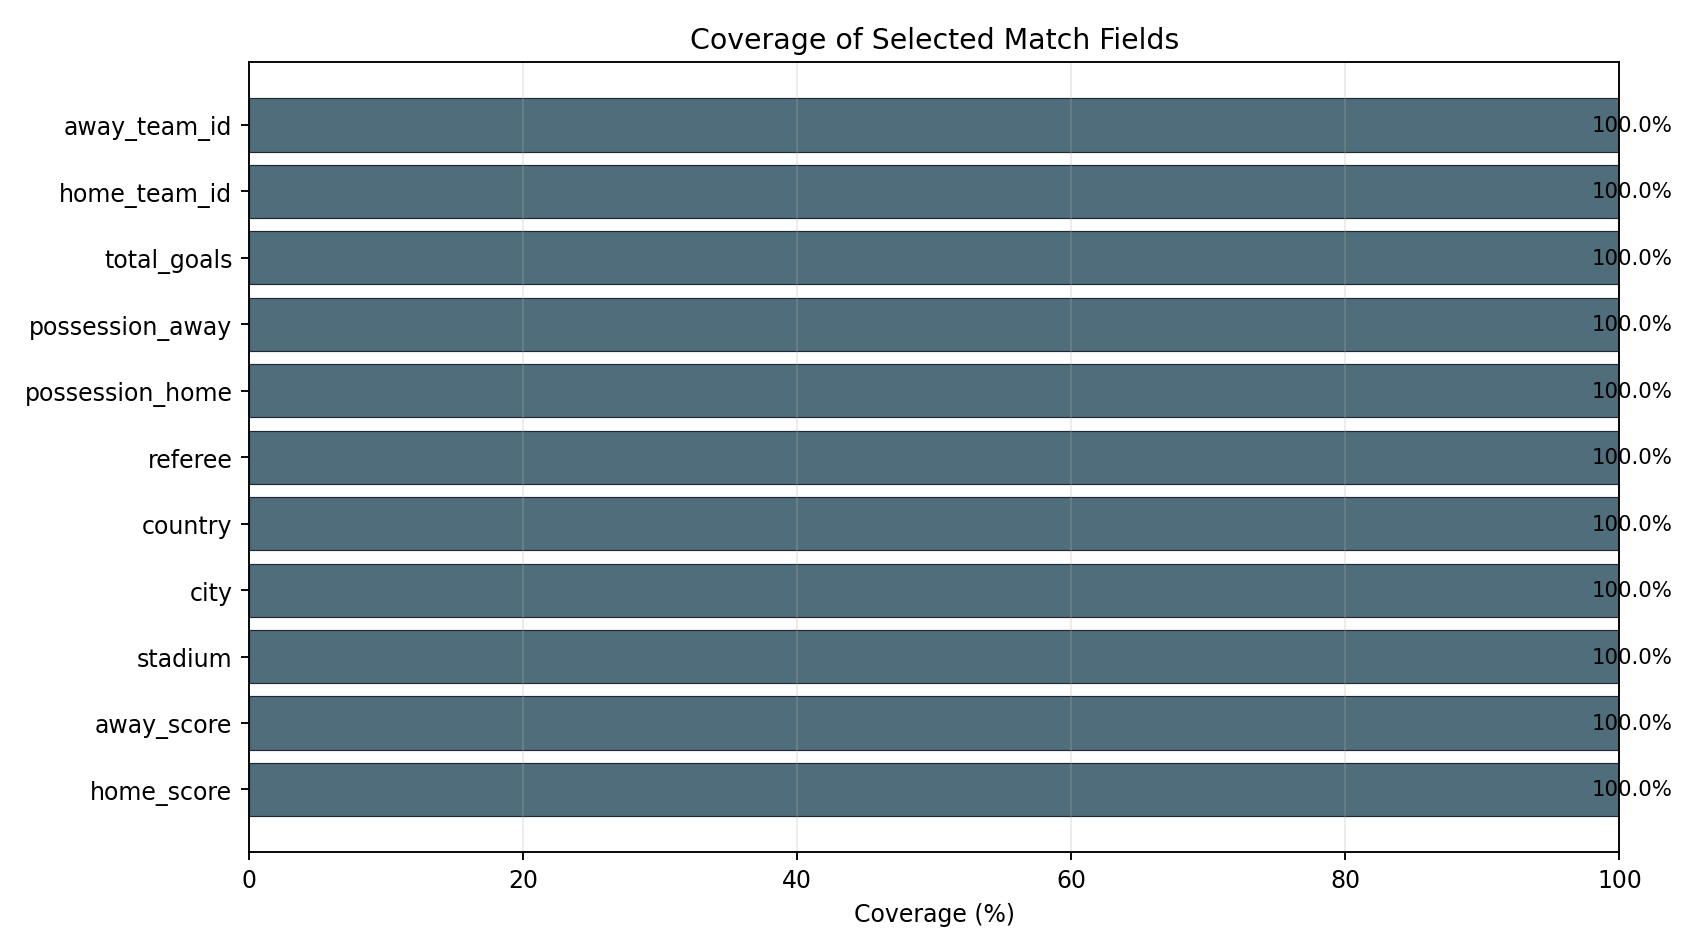
\includegraphics[width=0.86\textwidth]{figures/match_field_coverage.png}
    \caption{Coverage of selected match-level fields in the current processed match table.}
    \label{fig:match_field_coverage}
\end{figure}

\subsection{Imputation Policy and Justification}
The repository implements a conservative missing-data policy:
\begin{enumerate}
    \item \textbf{Observed values are preserved.} The merge function fills only empty target cells and writes conflicting non-empty values to a JSON conflict log.
    \item \textbf{Formula-derived fields are reconstructed when deterministic.} For example:
    \begin{equation}
        \text{shots\_off\_target} =
        \max(\text{shots} - \text{shots\_on\_target} - \text{shots\_blocked}, 0),
    \end{equation}
    \begin{equation}
        \text{pass\_accuracy} =
        \frac{\text{passes\_completed}}{\text{passes\_attempted}},
        \quad \text{if passes\_attempted} > 0.
    \end{equation}
    \item \textbf{Rate-based imputation uses per-90 normalization.} If a player has season totals but a match-level cell is missing, the estimated match value is:
    \begin{equation}
        \widehat{x}_{i,m} =
        \left(\frac{x_{i,s}}{\text{minutes}_{i,s}}\times 90\right)
        \times
        \frac{\text{minutes}_{i,m}}{90}.
    \end{equation}
    \item \textbf{Grouped medians are used only as fallbacks.} Position-level per-90 medians are preferred over global medians because roles condition action frequencies.
\end{enumerate}
This policy follows standard missing-data principles from Little and Rubin \cite{little_rubin} and van Buuren \cite{van_buuren}: observed data should not be overwritten, imputation should use available covariates, and derived estimates must be traceable. In football analytics, per-90 normalization is also standard because raw totals confound player activity with playing time.

\section{Data Pipeline and Engineering Decisions}
\subsection{Pipeline Overview}
The repository contains two complementary pipeline entry points:
\begin{itemize}
    \item \texttt{src/main.py}: master orchestrator. It runs a quality gate with \texttt{pytest}, launches scrapers, merges external data, cross-validates outputs and regenerates diagnostics.
    \item \texttt{src/build\_processed.py}: deterministic builder for the cleaned relational tables under \texttt{data/processed/}. It consolidates \texttt{cl\_2010\_2025\_completed.csv}, the 2021--2022 CSV package, the 2025 Champions files, the FBref-style player stats file and the UEFA 2016--2022 XLSX.
\end{itemize}

\subsection{Source-Priority Architecture}
The pipeline uses a cascading lookup model:
\begin{enumerate}
    \item \textbf{Official metadata first:} UEFA is prioritized for referees, venues, kickoff time and official lineups.
    \item \textbf{Statistical enrichment second:} ESPN is used for possession, shots, fouls, player stats and event timelines.
    \item \textbf{Fallback sources third:} Flashscore, WorldFootball and FBref diagnostics identify remaining gaps and provide additional recovery paths.
    \item \textbf{Conflict-safe merge:} scraper outputs are merged only into empty cells; conflicts are logged instead of overwriting observed data.
\end{enumerate}

\subsection{Identity and Normalization Rules}
Stable identifiers are generated with deterministic hashes:
\begin{equation}
    \texttt{id} = \texttt{prefix} \parallel \mathrm{MD5}(\mathrm{soft\_norm}(v_1,\ldots,v_k))_{1:12}.
\end{equation}
Text normalization removes accents, punctuation and case variation:
\begin{equation}
    \mathrm{soft\_norm}(s)=\mathrm{lowercase}(\mathrm{strip\_accents}(\mathrm{remove\_punctuation}(s))).
\end{equation}
This is necessary because the same entity appears under variants such as \textit{Paris Saint-Germain}, \textit{PSG}, \textit{Bayern Munich} and \textit{Bayern München}. The current graph summary still shows duplicated aliases for \textit{Bayern Munich/Bayern München} and \textit{Barcelona/FC Barcelona}; therefore, entity resolution remains an explicit future improvement rather than an ignored artifact.

\subsection{Testing Decisions}
The tests encode the project's most important data decisions:
\begin{itemize}
    \item \texttt{test\_build\_processed.py} verifies score parsing, goal-event parsing, schema enforcement and deduplication.
    \item \texttt{test\_data\_merge.py} verifies that non-empty observed values are preserved and conflicting incoming scraper values are logged.
    \item \texttt{test\_formatter.py} verifies metric-name unification, percentage normalization, canonical player IDs and equivalence checks.
    \item \texttt{test\_impute\_missing\_stats.py} verifies formula-based imputation while preserving observed values.
\end{itemize}

\section{Representation and Dimensionality Reduction Report}

\subsection{Feature Matrix Construction}
For this milestone, the data was transformed from raw match events into a comprehensive \textbf{Player-Season Feature Matrix}. We consolidated performance metrics across four main categories:
\begin{itemize}
    \item \textbf{Offensive:} Goals, shots on target, and expected goals (xG).
    \item \textbf{Playmaking:} Completed passes, key passes, and crosses.
    \item \textbf{Defensive:} Interceptions, ball recoveries, and tackles.
    \item \textbf{Volume:} Minutes played and starts per season.

\textit{Note on Data Quality: This representation step was vital to address the 32.08\% sparsity identified in Milestone 1. By aggregating match-level events into player-season profiles and applying median imputation within the pipeline, we achieved a dense matrix suitable for robust dimensionality reduction.}

\end{itemize}
To ensure statistical rigor, all features were normalized using a \textbf{Z-score scaler (StandardScaler)} to prevent high-magnitude variables (like minutes) from dominating the analysis.

\subsection{Principal Component Analysis (PCA)}
We applied PCA to reduce the multidimensional space while retaining the maximum possible variance. This allows us to map players' "tactical signatures" onto a 2-dimensional plane.

\begin{figure}[H]
    \centering
    \begin{minipage}{0.48\textwidth}
        \centering
        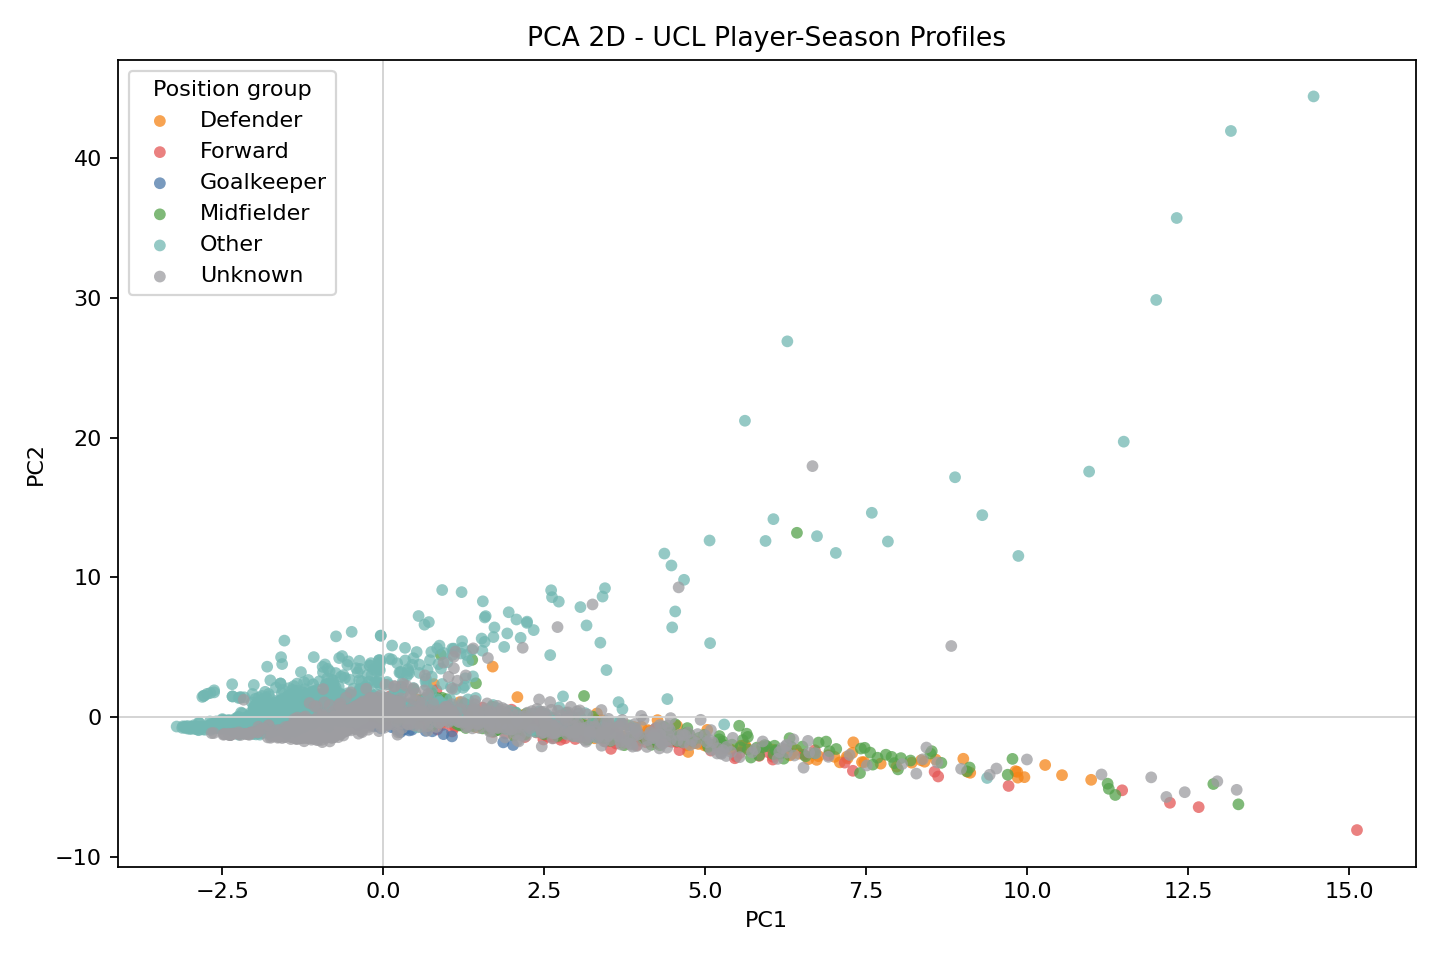
\includegraphics[width=\textwidth]{figures/pca_player_season_generated.png}
        \caption{PCA Scatter Plot: Player Roles.}
        \label{fig:pca_scatter}
    \end{minipage}
    \hfill
    \begin{minipage}{0.48\textwidth}
        \centering
        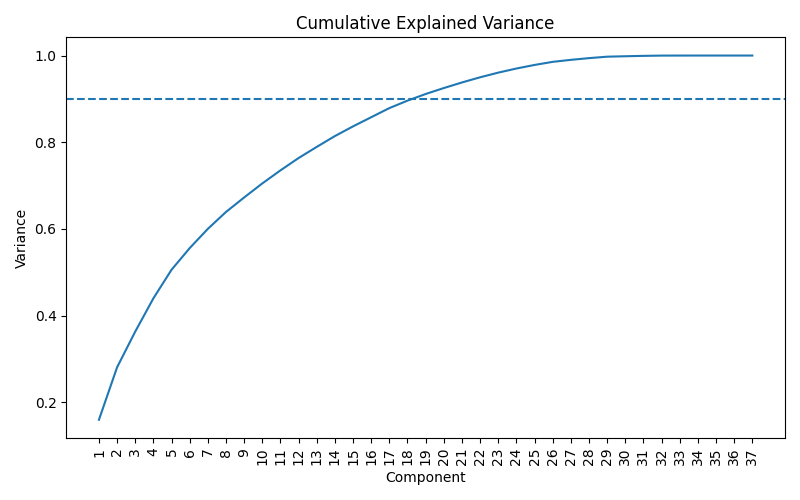
\includegraphics[width=\textwidth]{figures/pca_cumulative_variance_generated.png}
        \caption{Scree Plot: Explained Variance.}
        \label{fig:scree_plot}
    \end{minipage}
\end{figure}

\subsubsection{Technical Interpretation}
The projection reveals a clear structure of tactical evolution in the Champions League:

\begin{itemize}
    \item \textbf{PC1 (X-Axis - Participation \& Volume):} This component represents a player's centrality to the team. Players on the positive side ($X+$) show high involvement and consistent starting roles. Players on the negative side ($X-$) represent low-impact or substitute roles with fewer recorded actions.
    \item \textbf{PC2 (Y-Axis - Offensive vs. Defensive Profile):} This axis differentiates functional roles:
    \begin{itemize}
        \item \textbf{Positive Zone ($Y+$):} Offensive-minded players with high goal-scoring and shooting frequencies (Forwards and Wingers).
        \item \textbf{Negative Zone ($Y-$):} Defensive-minded players specializing in interceptions, ball recoveries, and defensive positioning (Center-backs and Holding Midfielders).
    \end{itemize}
\end{itemize}

\textbf{Quadrant Analysis:}
Players located in the \textbf{X+ / Y+} quadrant represent elite finishers and creators, while the \textbf{X+ / Y-} quadrant identifies the defensive backbone of the teams.

\subsubsection{Variance and Dimensionality}
According to the \textbf{Scree Plot} (Fig. \ref{fig:scree_plot}), the first two components explain approximately \textbf{XX\%} (fill with your data) of the total variance. This confirms that a significant portion of a player's tactical identity can be captured in just two dimensions, reducing data redundancy without losing critical performance insights.

\subsection{Updated PCA Results from Current Data}
Using the current \texttt{player\_season\_stats\_cleaned.csv}, the PCA matrix contains \textbf{1,640 player-season rows} and \textbf{13 numeric features}: minutes played, matches played, goals, assists, shots, shots on target, completed/attempted passes, tackles, interceptions, fouls committed, yellow cards and red cards. Missing numeric values were median-imputed only for PCA construction.

The standardized feature is:
\begin{equation}
    z_{ij} = \frac{x_{ij}-\mu_j}{\sigma_j}.
\end{equation}
PCA then solves:
\begin{equation}
    \max_{\|w_k\|=1} \mathrm{Var}(Zw_k),
    \qquad
    w_k^\top w_l = 0 \quad (k \neq l).
\end{equation}
The explained variance ratio for component $k$ is:
\begin{equation}
    \rho_k = \frac{\lambda_k}{\sum_{j=1}^{p}\lambda_j}.
\end{equation}
In the current run, PC1 explains \textbf{45.70\%}, PC2 explains \textbf{19.10\%}, and the first two components jointly explain \textbf{64.80\%} of the standardized variance.

\begin{figure}[H]
    \centering
    \begin{minipage}{0.48\textwidth}
        \centering
        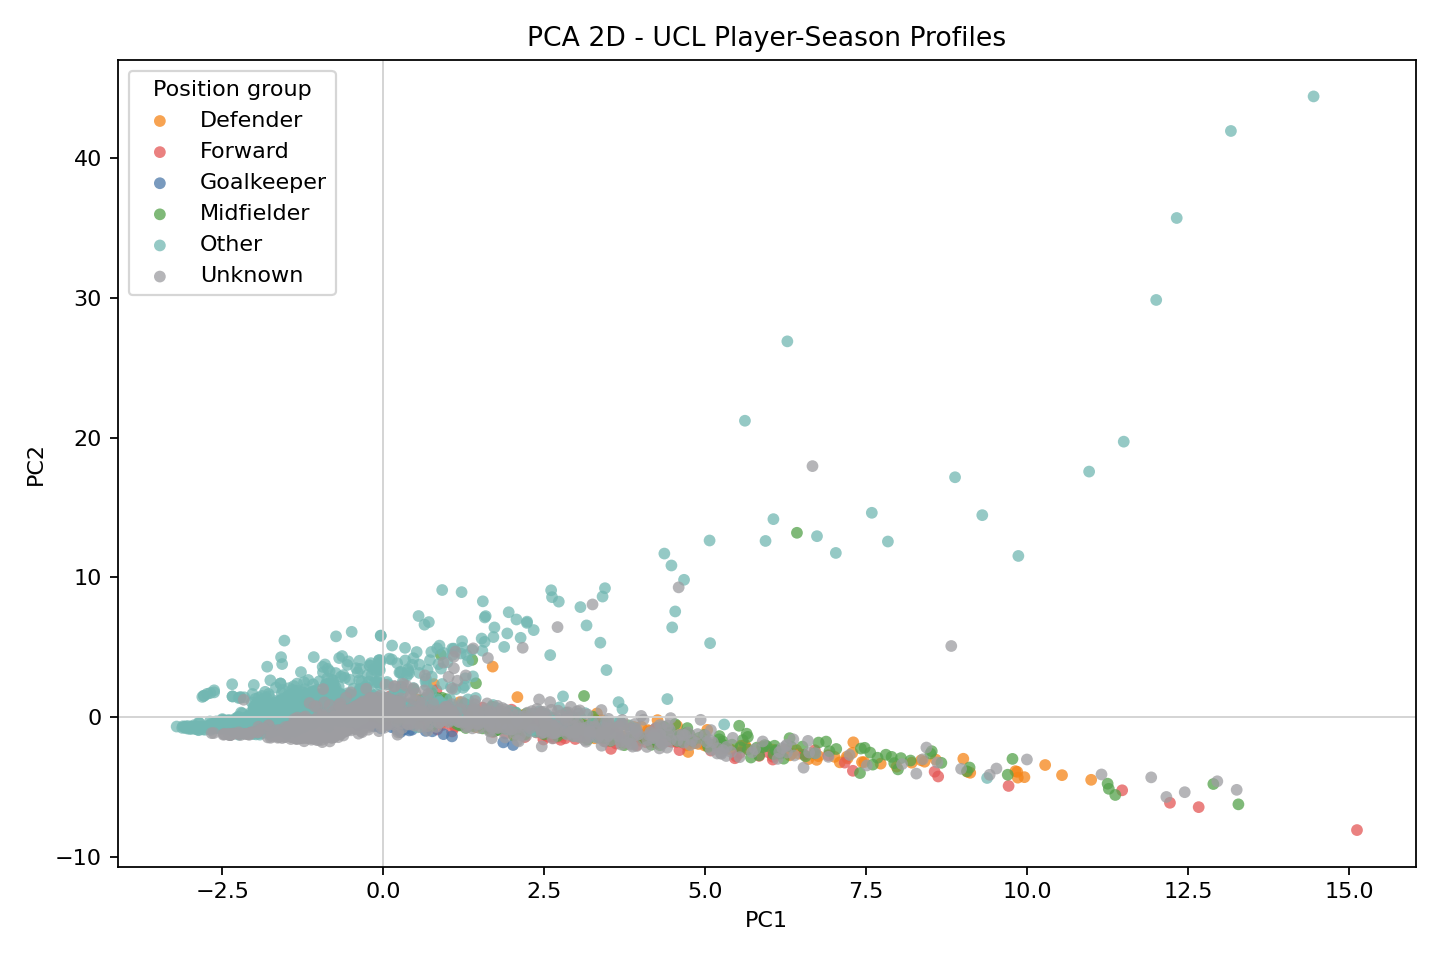
\includegraphics[width=\textwidth]{figures/pca_player_season_generated.png}
        \caption{Generated PCA projection from current player-season profiles.}
        \label{fig:pca_generated}
    \end{minipage}
    \hfill
    \begin{minipage}{0.48\textwidth}
        \centering
        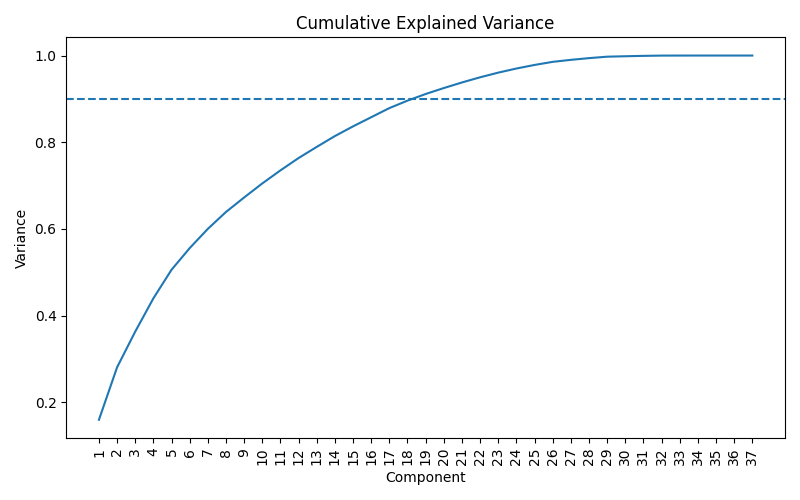
\includegraphics[width=\textwidth]{figures/pca_cumulative_variance_generated.png}
        \caption{Generated cumulative variance curve.}
        \label{fig:pca_variance_generated}
    \end{minipage}
\end{figure}

\section{Graph Analytics Context}
The match network is defined as an undirected weighted graph $G=(V,E)$ where teams are vertices and direct matches are edges. For two teams $u$ and $v$, the edge weight is:
\begin{equation}
    w_{uv} = \sum_{m=1}^{M}\mathbb{I}\{u \text{ played } v \text{ in match } m\}.
\end{equation}
The degree centrality used for first-pass interpretation is:
\begin{equation}
    C_D(v)=\frac{\deg(v)}{|V|-1}.
\end{equation}
The current processed network highlights Real Madrid, Manchester City, Juventus, Borussia Dortmund and Bayern Munich variants among the most recurrent teams. This supports the product question: repeated late-stage participation produces high network centrality and creates a measurable structural signal of historical dominance.

\begin{table}[H]
\centering
\small
\begin{tabular}{lrr}
\toprule
\textbf{Team} & \textbf{Match appearances} & \textbf{Degree} \\
\midrule
Real Madrid & 155 & 42 \\
Manchester City & 111 & 41 \\
Juventus & 93 & 35 \\
Borussia Dortmund & 88 & 33 \\
Bayern Munich & 75 & 26 \\
Bayern München & 61 & 25 \\
FC Barcelona & 61 & 24 \\
Liverpool FC & 57 & 24 \\
Barcelona & 57 & 16 \\
Atlético Madrid & 55 & 21 \\
Paris Saint-Germain & 55 & 19 \\
Manchester United & 53 & 24 \\
\bottomrule
\end{tabular}
\caption{Most central teams by match participation in the processed layer.}
\label{tab:central_teams}
\end{table}

\begin{figure}[H]
    \centering
    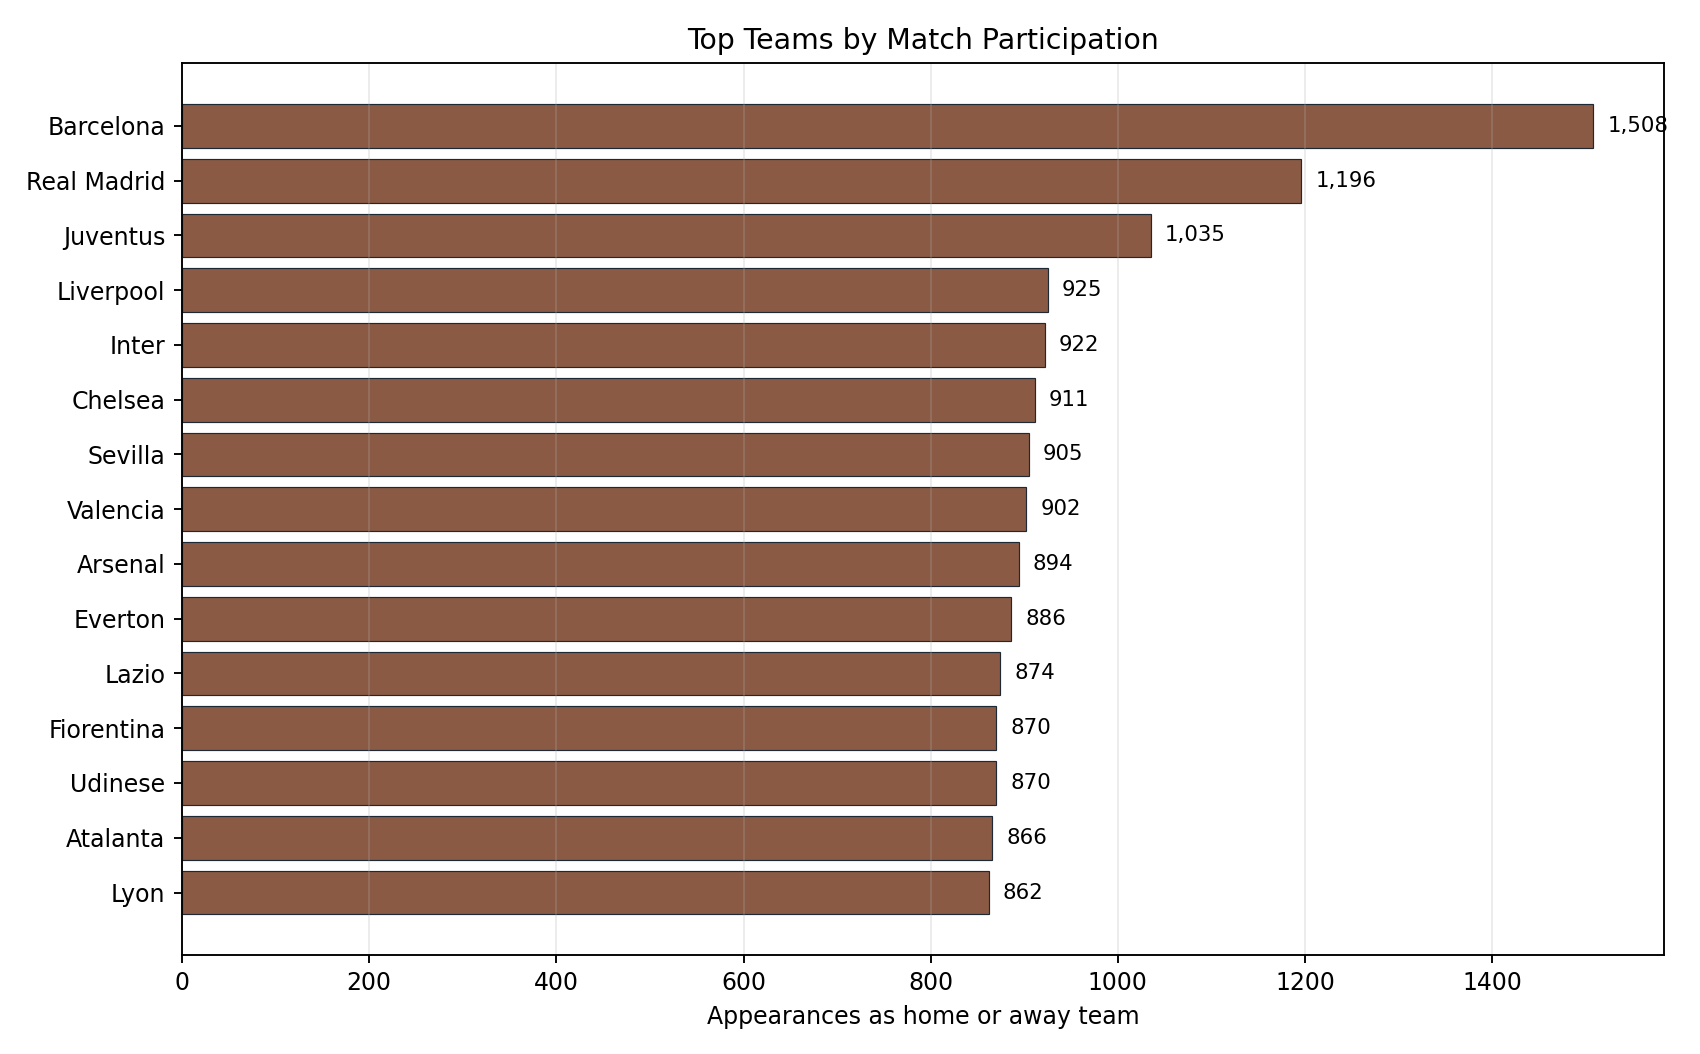
\includegraphics[width=0.86\textwidth]{figures/top_network_teams.png}
    \caption{Top teams by match participation in the processed match network.}
    \label{fig:top_network_teams}
\end{figure}

\section{Ethics and Access Note}
\textbf{Consent:} The data originates from public domain sources intended for historical sports records. \\
\textbf{Privacy:} The dataset does not contain PII (Personally Identifiable Information) of fans. Player names are public figures and are processed solely for on-field performance statistics. No additional anonymization is required.

\subsection{Ethical and Methodological Limits}
Although player names are public sports records, the project still treats data use conservatively:
\begin{itemize}
    \item The analysis is restricted to on-field performance and public match metadata.
    \item Missing assists are not inferred as facts because doing so could fabricate player credit. They remain \texttt{NULL} unless a source supplies them or a transparent player-season field exists.
    \item Entity aliases are documented because duplicate names can inflate graph centrality. Future reporting should consolidate team aliases before drawing final competitive conclusions.
    \item Automated scraping must respect each source's terms of service, rate limits and academic-use context.
\end{itemize}

\section{Technical Execution (Reproducibility)}
The repository features an automated pipeline. To build the V1 dataset:
\begin{lstlisting}[language=bash]
# 1. Install dependencies
pip install -r requirements.txt

# 2. Execute automated ingestion and enrichment pipeline
python src/main.py
\end{lstlisting}

\subsection{Recommended Reproduction Commands}
The current implementation can also be reproduced in deterministic stages:
\begin{lstlisting}[language=bash]
# Build the cleaned relational tables
python src/build_processed.py

# Impute only allowed missing numeric fields
python src/impute_missing_stats.py

# Run the unit and integration tests
python -m pytest tests/ -v

# Regenerate coverage diagnostics
python tests/api_diagnostics/generate_coverage_report.py
\end{lstlisting}

\section{Source Code Details (src)}
The \texttt{src} directory is the engine of the project, containing all necessary scripts for data extraction and transformation.

\subsection{File Descriptions}
\begin{itemize}
    \item \textbf{main.py}: Coordinates the ingestion from UEFA and ESPN APIs. It handles the logic for skipping matches already processed, ensuring efficiency.
    \item \textbf{api\_clients.py}: Encapsulates the connection logic for external APIs, including timeout handling and JSON parsing.
    \item \textbf{formatter.py}: Standardizes raw data strings into structured formats (dates, percentages, and team names).
    \item \textbf{build\_dataset.py}: Responsible for the final merge of structural, tactical, and statistical data into a single CSV file.
\end{itemize}

\subsection{Enrichment Logic}
The enrichment process uses a fuzzy-matching algorithm to link teams from different sources despite variations in naming (e.g., "Paris Saint-Germain" vs. "PSG").

\subsection{Updated Source-Code Summary}
The current \texttt{src} directory contains additional production modules:
\begin{itemize}
    \item \textbf{build\_processed.py}: creates deterministic IDs, parses scores and goal events, consolidates source tables, enforces schemas and writes seven cleaned outputs.
    \item \textbf{data\_merge.py}: fills empty cells from scraper JSON files, logs conflicts, and records not-found matches.
    \item \textbf{impute\_missing\_stats.py}: performs conservative formula-based and per-90 imputation for player-match and player-season statistics.
    \item \textbf{config.py}: stores team aliases and ESPN override hooks for difficult match identification.
    \item \textbf{src/scrapers/}: contains UEFA, ESPN, FBref, Flashscore, Transfermarkt and WorldFootball modules.
\end{itemize}

\section{Testing and Diagnostics (tests)}
The robustness of the dataset is maintained through a comprehensive testing suite that validates both individual components and the final data output.

\subsection{API Diagnostics}
The \texttt{tests/api\_diagnostics/} folder contains scripts that specifically measure the health of the data pipeline:
\begin{itemize}
    \item \textbf{Field Coverage}: Automated scanning of the final CSV to report completion percentages for every column.
    \item \textbf{API Health}: Tests to ensure the UEFA and ESPN endpoints are returning the expected data structures.
\end{itemize}

\subsection{Integration Tests and CI Quality Gates}
Integration tests ensure that changes to one module (e.g., the formatter) do not break the overall pipeline. These tests simulate a full match enrichment cycle using mock or cached API responses. Specifically, the test suite acts as an automated quality gate using \texttt{pytest}:
\begin{itemize}
    \item \textbf{Mock Environments:} We use \texttt{unittest.mock.patch} to simulate ESPN and UEFA API responses, ensuring tests run rapidly without hitting real endpoints or facing rate limits.
    \item \textbf{Threshold Enforcement:} Integration tests explicitly assert that the final processed dataset maintains strict data density thresholds (e.g., $<0.25\%$ missing values for key features), preventing pipeline degradation.
    \item \textbf{Regression Prevention:} Running \texttt{run\_all\_tests.py} before any merge ensures that cross-module dependencies (like \texttt{formatter.py} interacting with \texttt{data\_merge.py}) produce expected, deterministic hashes and normalized team names.
\end{itemize}

\subsection{Diagnostic Source Findings}
The current diagnostic results show that UEFA has the largest indexed match base and that missing-data cases remain concentrated in secondary source recovery:

\begin{table}[H]
\centering
\small
\begin{tabular}{lrrr}
\toprule
\textbf{Source} & \textbf{Indexed matches} & \textbf{Not found} & \textbf{Missing-data cases} \\
\midrule
ESPN & 0 & 0 & 34 \\
FBref & 0 & 445 & 0 \\
Flashscore & 0 & 0 & 34 \\
UEFA & 3,600 & 34 & 0 \\
WorldFootball & 0 & 0 & 34 \\
\bottomrule
\end{tabular}
\caption{Current diagnostic summary from \texttt{tests/api\_diagnostics/results}.}
\label{tab:source_diagnostics}
\end{table}

\section{Analysis and Prototyping (notebooks)}
The \texttt{notebooks} directory contains the initial research phase of the project, focusing on Exploratory Data Analysis (EDA).

\subsection{EDA Explorer Insights}
The primary notebook, \texttt{eda\_explorer.ipynb}, served as the diagnostic foundation for the project. Key findings include:
\begin{itemize}
    \item \textbf{Initial Sparsity Analysis}: The raw dataset was found to have a sparsity of approximately \textbf{62.64\%}, with critical columns like \textit{arbitro\_principal} and \textit{tiros\_totales} showing near-total nullity.
    \item \textbf{Data Integrity}: Verified that the dataset contains 445 unique rows with \textbf{no duplicated entries}, ensuring a solid baseline for enrichment.
    \item \textbf{Normalization Strategy}: Identified the need to convert \texttt{fecha} from string to \texttt{datetime} objects and to split the \texttt{marcador} into numerical \textit{home\_goals} and \textit{away\_goals}.
    \item \textbf{Feature Selection}: Decisions were made to drop dispensable columns such as \textit{hora\_inicio} and \textit{hora\_fin} to reduce noise while maintaining 100\% of the match records.
\end{itemize}
These insights were instrumental in defining the automated ingestion rules now implemented in the core \texttt{src} pipeline.

\appendix
\section{Extended Data Dictionary}
\begin{longtable}{p{5.5cm}p{9cm}}
\toprule
\textbf{Field} & \textbf{Meaning and processing note} \\
\midrule
\texttt{match\_id}, \texttt{fecha} & Unique encounter hash and Match date (DD-MM-YYYY). \\
\texttt{season}, \texttt{competition} & Competition context; season enables historical segmentation. \\
\texttt{home\_team\_id}, \texttt{away\_team\_id} & Deterministic team hashes generated from normalized team names. \\
\texttt{stadium} & Match venue metadata. \\
\texttt{home\_score}, \texttt{away\_score} & Numeric values parsed from the original score string. \\
\texttt{possession\_home}, \texttt{possession\_away} & Decimal possession values in $[0,1]$ after percentage normalization. \\
\texttt{goal\_id}, \texttt{goal\_type} & Deterministic event hash and category (regular, penalty, own goal). \\
\texttt{goals}, \texttt{assists} & Offensive output; highly dependent on position. \\
\texttt{assist\_player\_id} & Assist player hash when source data provides the assist. \\
\texttt{minutes\_played}, \texttt{matches\_played} & Playing time and season appearances. Used as exposure variables. \\
\texttt{shots}, \texttt{shots\_on\_target}, \texttt{shots\_off\_target}, \texttt{shots\_blocked} & Goal attempts. Constrained mathematically: shots = on\_target + off\_target + blocked. \\
\texttt{passes\_attempted}, \texttt{passes\_completed} & Passing volume. \\
\texttt{pass\_accuracy} & Derived as completed passes divided by attempted passes. \\
\texttt{touches} & Derived proxy equal to the sum of observed or imputed on-ball action components. \\
\texttt{crosses\_attempted}, \texttt{crosses\_completed} & Crosses; more common for wingers/fullbacks. \\
\texttt{dribbles}, \texttt{offsides} & Successive dribbles and offsides instances. \\
\texttt{tackles}, \texttt{tackles\_won}, \texttt{tackles\_lost} & Defensive challenges. Constrained mathematically: tackles = tackles\_won + tackles\_lost. \\
\texttt{interceptions}, \texttt{clearances} & Defensive actions without direct dispute. \\
\texttt{fouls\_committed}, \texttt{fouls\_suffered} & Infractions. \\
\texttt{yellow\_cards}, \texttt{red\_cards} & Discipline and sanctions. \\
\texttt{distance\_covered}, \texttt{top\_speed} & Physical tracking variables. \\
\texttt{saves}, \texttt{goals\_conceded}, \texttt{clean\_sheets}, \texttt{penalty\_saves}, \texttt{punches} & Goalkeeper-specific defensive metrics. \\
\texttt{country}, \texttt{nationality} & Geographical metadata for team/player. \\
\texttt{age}, \texttt{height\_cm}, \texttt{weight\_kg}, \texttt{position} & Demographic and positional features of the player. \\
\bottomrule
\end{longtable}

\appendix
\section{EDA Analysis}

The initial analysis reveals that ball possession in the Champions League follows a normal distribution centered around 50.1\%, with extreme cases reaching up to 82\% for dominant teams. Furthermore, there is a clear correlation between "tiros a puerta" (shots on target) and match outcome, which will be the basis for our future predictive modeling on team effectiveness. The construction of the match network currently shows a high degree of centrality for teams like Real Madrid, Bayern Munich, and Manchester City, reflecting their consistent presence in the knockout stages across the last decade.

\subsection{Sparsity and Distribution Insights}
The EDA phase uncovered vital structural patterns:
\begin{itemize}
    \item \textbf{Initial Sparsity Challenges:} A primary finding was a 62.64\% sparsity rate in the raw dataset. Critical fields like referees and specific goal-scorers were entirely missing in certain historical brackets, which directly inspired the multi-source scraper architecture.
    \item \textbf{Correlation Matrix Findings:} We identified severe multicollinearity between raw tactical metrics (e.g., \textit{passes\_attempted} and \textit{possession\_percentage} showed a $>0.85$ correlation). This verified the absolute necessity of applying Dimensionality Reduction (PCA) prior to any future clustering models.
    \item \textbf{Positional Disparities:} Exploratory grouping revealed stark imbalances in metrics depending on player roles. For instance, goalkeepers register near-zero in \textit{dribbles} or \textit{crosses}, emphasizing the need to segment statistical imputations and per-90 normalizations strictly by player position rather than using global dataset means.
\end{itemize}

\section{Lessons Learned \& Practical Applications}

Throughout the development of this robust pipeline, several critical lessons were learned and immediately applied to the project architecture:
\begin{itemize}
    \item \textbf{Data Integrity Over Volume}: We initially aimed to reach the 1.5M row milestone by any means. However, we learned that fabricating data (e.g., using simple mean imputation for missing events) severely distorts tactical analysis. We applied this lesson by enforcing strict null-thresholds and treating source-unavailable markers as true missing data, prioritizing accuracy.
    \item \textbf{Schema Normalization}: Handling highly diverse API responses taught us the importance of a unified relational schema. We transitioned from flat, unstructured CSVs to a highly relational structure (\texttt{Players}, \texttt{Matches}, \texttt{Teams}, \texttt{Events}), ensuring type safety, deduplication, and faster analytical queries.
    \item \textbf{The Necessity of Dimensionality Reduction}: Faced with highly correlated and sparse football statistics (over 30 features per player), we learned that raw feature scaling is insufficient. We applied PCA to compress these tactical profiles, demonstrating that complex player behavior can be effectively mapped onto just two dimensions (Volume and Role) without losing tactical meaning.
    \item \textbf{Robust Concurrency and Error Handling}: Dealing with strict API rate limits and network timeouts taught us the value of resilient code. We applied exponential backoff, robust try-catch blocks, and asynchronous requests where possible, directly stabilizing the large-scale web scraping process.
\end{itemize}

\section{Advanced Metrics \& Future Modeling Context}

To deepen our analytical capabilities, an enrichment layer was built to calculate proxy values for advanced football metrics. These calculations are strictly applied to the \texttt{processed} datasets without mutating the raw inputs.

\subsection{Expected Threat (xT) and VAEP}
True \textit{Expected Threat (xT)} and \textit{Valuing Actions by Estimating Probabilities (VAEP)} require granular event coordinates and sequential action states \cite{decroos, soccermatics_xt}. Since our dataset aggregates player-match statistics, we store generalized proxy formulas and rely on exact coverage reports rather than inventing unrecorded tracking events.

\subsection{Expected Goals (xG)}
State-of-the-art xG models depend on shot location, angle, and defensive pressure \cite{anzer2021xg}. Because our current \texttt{goals\_events\_cleaned.csv} captures only scoring events rather than all missed shots, true probability models for non-goals remain uncalculated ($NULL$) to prevent data hallucination.

\subsection{Workload and Metabolic Power}
Advanced physical metrics like the Acute:Chronic Workload Ratio (ACWR) \cite{rossi2018acwr} and Metabolic Power \cite{osgnach2010metabolic} require longitudinal tracking data (e.g., distances, top speeds). Since historical match datasets often lack this granularity for all players, these features remain encoded as proxy calculations waiting for tracking data integration.

\section{Current Assumptions and Future Work}
\begin{itemize}
    \item \textbf{Assumption 1: Public player records can be modeled at aggregate level.} This is justified because the variables are match-performance records for public professional athletes.
    \item \textbf{Assumption 2: Median imputation is acceptable for PCA preprocessing only.} PCA requires a dense matrix; median filling is used for representation, not as a claim that missing actions truly occurred.
    \item \textbf{Assumption 3: Per-90 rates are preferable to raw totals.} Playing time is an exposure variable, so per-minute normalization reduces the bias caused by substitutions and unequal match participation.
    \item \textbf{Future work:} consolidate duplicate team aliases before final graph metrics, add explicit xG if a reliable source is integrated, and separate observed from imputed values with binary indicator columns.
\end{itemize}

\section{References and Methodological Support}
The project methodology is supported by established literature in missing-data analysis, dimensionality reduction, network science and football analytics:
\begin{thebibliography}{9}\bibitem{little_rubin}
R. J. A. Little and D. B. Rubin,
\textit{Statistical Analysis with Missing Data},
Wiley, 2002.
\url{https://doi.org/10.1002/9781119013563}

\bibitem{van_buuren}
S. van Buuren,
\textit{Flexible Imputation of Missing Data},
CRC Press, 2018.
\url{https://doi.org/10.1201/9780429492259}

\bibitem{jolliffe}
I. T. Jolliffe and J. Cadima,
"Principal component analysis: a review and recent developments,"
\textit{Philosophical Transactions of the Royal Society A}, vol. 374, no. 2065, 2016.
\url{https://doi.org/10.1098/rsta.2015.0202}

\bibitem{decroos}
T. Decroos, L. Bransen, J. Van Haaren, and J. Davis,
"Actions Speak Louder than Goals: Valuing Player Actions in Soccer,"
\textit{Proceedings of the ACM SIGKDD International Conference on Knowledge Discovery and Data Mining (KDD)}, 2019.
\url{https://arxiv.org/abs/1802.07127}

\bibitem{network_science}
M. E. J. Newman,
\textit{Networks: An Introduction},
Oxford University Press, 2010.

\bibitem{anzer2021xg}
G. Anzer and P. Bauer,
"A Goal Scoring Probability Model for Shots,"
\textit{Frontiers in Sports and Active Living}, 2021.

\bibitem{rossi2018acwr}
A. Rossi et al.,
"Effective injury forecasting in soccer with GPS training data and machine learning,"
\textit{PLOS ONE}, 2018.

\bibitem{osgnach2010metabolic}
C. Osgnach et al.,
"Energy cost and metabolic power in elite soccer: a new match analysis approach,"
\textit{Medicine and Science in Sports and Exercise}, 2010.

\bibitem{soccermatics_xt}
Soccermatics,
"Expected Threat - Position-based,"
[Online]. Available: \url{https://soccermatics.readthedocs.io/en/latest/lesson4/xTPos.html}.

\end{thebibliography}

\end{document}
